\documentclass[handout]{beamer}
\usepackage{multirow}
\usepackage{rotating}
\usepackage{fontspec} 
\usepackage{booktabs}
% \usepackage{lsp-makros}
\useoutertheme{lsp}

\usepackage{lsptitle}

\def\two@digits#1{\ifnum#1<10 0\fi\number#1}
\def\mytoday{\two@digits{\number\day}.\two@digits{\number\month}.\number\year}


\usepackage{xspace,multicol}
\newcommand{\latex}{\LaTeX\xspace}
\usepackage{tikz}


\newcounter{lastpagemainpart}
\footnotesep0pt
\renewcommand{\footnoterule}{}
\usefootnotetemplate{
  \noindent
  \insertfootnotemark\insertfootnotetext}

\let\beamerfn=\footnote
\renewcommand{\footnote}[1]{%
\let\oldfnsize=\footnotesize%
\let\footnotesize=\tiny%
\beamerfn<\thebeamerpauses->{#1}%
\let\footnotesize=\oldfnsize}


\date{\today}

\usepackage{eurosym}  
 
\renewcommand{\centerline}[1]{\hfill#1\hfill\hfill\mbox{}}


\title{Language Science Press business model\newline {\small \url{bit.ly/3fJ1AF7}}}
% \institute{FU Berlin}
\author[LangSci]{Sebastian Nordhoff}



\begin{document}
\lspbeamertitle

\section{Introduction}
\frame{
\frametitle{Introduction LangSci Press}
%   \includegraphics[height=.2\textheight]{./path/to/graphicsfile}
  \begin{itemize}
    \item  founded 2014
    \item Diamond OA
    \item only books, only linguistics, only CC-BY
    \item 150 books published (1\,000+ authors)
    \begin{itemize}
        \item 1\,187\,932 downloads as of January 2021
      \item top books at 60k downloads
    \end{itemize}
  \end{itemize}
  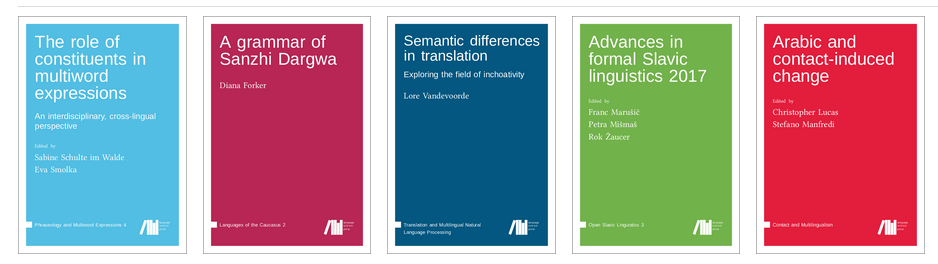
\includegraphics[height=3cm]{seriesbooks.png}
}

\frame{
\frametitle{Introduction LangSci Press}
\begin{columns}
  \begin{column}{8cm}
  \begin{itemize}
    \item  discipline-specific
    \item international
    \item values: \textbf{excellence}, \textbf{transparency}, \textbf{collaboration}
    \item initial grant had a position for an economist
    \item read the \textit{Cookbook for Open Access books}   and our annotated business model
    \item available on \url{https://langsci-press.org/opendata}
  \end{itemize}
  \end{column}
  \begin{column}{2cm}
  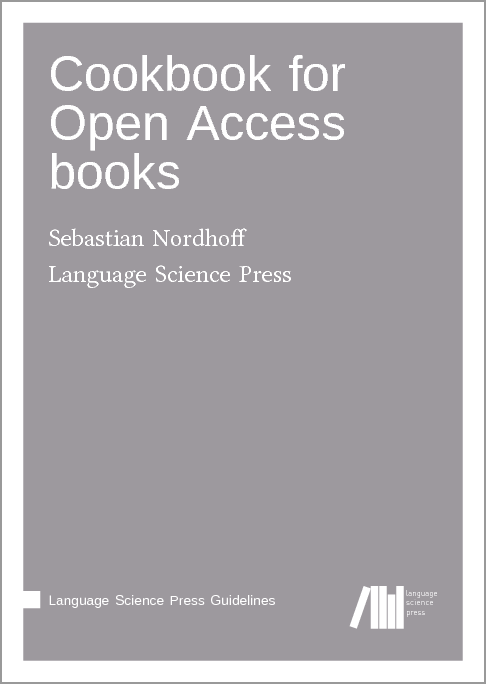
\includegraphics[height=3cm]{cookbook.png}
  
\includegraphics[height=3cm]{businessmodel.png}
  \end{column}
\end{columns}
}



\section{Revenue}
\frame{
\frametitle{Revenue 2020}
%   \includegraphics[height=.2\textheight]{./path/to/graphicsfile}
  \begin{itemize}
    \item 113k€ revenue
    \begin{itemize}
      \item 105k€ \textbf{consortial funding} via Knowledge Unlatched
      \item 8k€ varia
      \begin{itemize}
        \item  print margin, donations, BPCs
      \end{itemize}
    \end{itemize}
    \item funding 2018-2020:                 105 institutions (1\,000€/year)
    \item funding 2021-2023:                 115 institutions (1\,000€/year)
    \item the revenue streams of \textbf{private donations}, \textbf{private memberships}, \textbf{BPCs}, \textbf{print margins} have all been investigated, but they do not yield sufficient amounts of money
  \end{itemize}
}

\section{Costs}
\frame{
\frametitle{Costs}
\begin{columns}
\begin{column}{6cm}
  \begin{itemize}
    \item  120k€
    \begin{itemize}
      \item   90k€ salaries
      \item   6k€ rent
      \item   20k€ service providers
    \end{itemize}
    \item no warehousing, no marketing, no paywall maintenance, \\no royalties, no legal department, no invoicing
  \end{itemize}
  \end{column}
  \begin{column}{4cm}
    \hspace*{-1cm}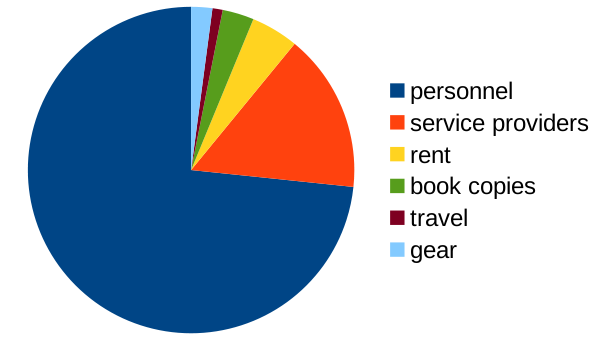
\includegraphics[width=6cm]{costtypes2020.png}
  \end{column}
  \end{columns}

}

\section{Legal issues}


\frame{
\frametitle{Legal form}
\begin{itemize}
  \item different legal forms have different advantages with regard to flexibility and not-for-profit branding
\end{itemize}
\bigskip
\large\color{lsDarkBlue}
\begin{tabular}{|lp{4mm}@{~}|p{3cm}|p{6cm}|}
\hline
&  &\multicolumn{2}{c|}{\textbf{commercial~~~~~~~~~~~~~~~~~~~}}\\
&  & \multicolumn{1}{c}{+} & \multicolumn{1}{c|}{--}\\
  \hline
\multirow{2}{*}{\begin{sideways}{\textbf{flexible}~~~~~~~}\end{sideways}}
&~\newline-- & & Uni\newline~\newline Verein ($\approx$association) \\
\cline{3-4}
&~\newline+ & GmbH ($\approx$Ltd.)\newline~\newline \mbox{UG ($\approx$micro-Ltd)} &  \textbf{gUG ($\approx$charitable micro-Ltd)}\\
\hline
  \end{tabular}
\bigskip
  \begin{itemize}
    \item This varies greatly between jurisdictions. The above holds true for Germany only!
  \end{itemize}

}

\frame{
\frametitle{Brand}
  \begin{itemize}
    \item we have registered our trademark/logo
    \item secure your brand!
    \item don't sell your brand!
  \end{itemize}
}

\section{Workflows}
\frame{
\frametitle{Workflows: production}
%   \includegraphics[height=.2\textheight]{./path/to/graphicsfile}
  \begin{itemize}
    \item  community based
    \begin{itemize}
      \item 29 autonomous series (peer review)
      \item 400+ community proofreaders
    \end{itemize}
    \item streamlined and automated workflow
    \begin{itemize}
      \item standard templates (docx and tex)
      \item no XML
      \item docx$\to$tex conversion pipeline
      \item \LaTeX $\to$ pdf
      \item collaborative production on Overleaf
      \item print-on-demand via BoD
    \end{itemize}
  \end{itemize}
}

\frame{
\frametitle{Automation}
%   \includegraphics[height=.2\textheight]{./path/to/graphicsfile}
We automate most processes as far as we can
      \begin{itemize}
        \item doc2tex conversion
        \item checking of adherence to guidelines
        \item upload to Zenodo
        \item upload to print-on-demand
        \item report generation
      \end{itemize}
We are lucky to have sufficient programming expertise in-house
}


 \frame{
\frametitle{Dissemination}
%   \includegraphics[height=.2\textheight]{./path/to/graphicsfile}
  \begin{itemize}
    \item Digital versions are available via
    \begin{itemize}
      \item langsci-press.org, Zenodo, DOAB, OAPEN, GitHub, Paperhive. GoogleBooks, EBSCO, Scopus
    \end{itemize}
    \item printed books are available via
    \begin{itemize}
      \item VLB, your local book store, Amazon
    \end{itemize}
    \item books are announced on Twitter, Facebook, LinguistList, discipline-specific mailinglists.
    \item we sell about 500 books a year and have about 500k pdf downloads a year (excluding robots)
  \end{itemize}
}

\frame{
\frametitle{KOALA}
%   \includegraphics[height=.2\textheight]{./path/to/graphicsfile}
  \begin{itemize}
    \item project at the Technische Informationsbibliothek Hannover
    \item  Koala = \textbf{K}onsortiale \textbf{OA} \textbf{L}ösungen \textbf{a}ufbauen
    \begin{itemize}
        \item  = establishing consortial OA solutions
    \end{itemize}
    \item goal: \textbf{provide a blueprint for consortial funding for scholar-led presses}
    \item looking for: \textbf{presses interested in becoming a pilot project}
    \item \url{https://projects.tib.eu/koala}
    \item sebastian.nordhoff@tib.eu
  \end{itemize}
  
\includegraphics[height=2cm]{koala.jpg}
}

\end{document}
